\section{考察}

\subsection{採用したインタフェース設計について}

\subsubsection{検索を関数呼び出し演算子とする設計}

検索を {\tt operator()} の多重定義としたことには，記法上の利点と設計上の利点がある．記法上は，ハッシュ表が数学的にはキーから値への部分写像であることを踏まえると，{\tt table("hoge")} という「写像の適用」の形で検索を書けるのは自然である．設計上は，戻り値を {\tt const T*} とし「無し」を {\tt nullptr} で表現したことで，任意の型 {\tt T} に対して番兵値を用意することなく成否と値を同時に返せる．

一方，C++ の標準ライブラリの連想コンテナ {\tt std::map} は検索・挿入を兼ねる {\tt operator[]} を提供するが，この演算子は未登録キーへのアクセスで既定値の要素を自動的に挿入するという副作用をもつ．本実装の {\tt operator()} は const メンバ関数であり，検索によって表の状態が変化することはない．検索操作が表を書き換えないという性質が型システムで保証される点で，本設計は {\tt operator[]} 方式よりも誤用しにくいと考えられる．ただし，ポインタを返す設計には，返されたポインタの寿命が対象要素の寿命に従属するという注意点がある．すなわち当該キーが削除された後にポインタを参照すると未定義動作となる．この危険は {\tt hash.c} の {\tt find} が返すポインタにも同様に存在するものであり，ポインタを長期間保持しないという利用規約で回避する設計とした．

\subsubsection{削除を複合代入演算子とする設計}

削除を {\tt operator-=} としたことで，「表からキーを引き去る」という直感に沿った記法 {\tt table -= "hoge"} が得られた．演算子の意味論として，組込み型の {\tt -=} と同様に自オブジェクトへの参照を返すため，{\tt (table -= "a") -= "b"} のような連鎖適用も可能である．一般の設計では {\tt erase} のような名前付きメンバ関数のほうが意図が明瞭であるという立場もあるが，演算子多重定義は「本来の演算子の意味から類推できる場合に限って用いる」という指針に照らすと，集合からの要素の除去を減算と見なす本設計はその範囲に収まっていると考えられる．なお，削除が実際に行われたかどうかを呼び出し側が知る手段として，本実装では削除前後の {\tt size()} の比較が利用できる．

\subsubsection{テンプレート化の効果と限界}

テンプレート化により，値の型ごとにクラスを書き直すことなく {\tt HashTable<int>}，{\tt HashTable<double>}，{\tt HashTable<std::string>} が同一のソースから得られた（4.2 節）．C 言語で同等の汎用性を得るには，{\tt void*} と明示的キャストを使うか，マクロでコードを複製するかのいずれかになるが，前者は型安全性を失い（誤った型へのキャストがコンパイル時に検出されない），後者はデバッグが困難になる．テンプレートはコンパイラが型ごとに専用コードを生成するため，型安全性と実行効率を両立できる．

一方で限界も観察された．第一に，テンプレートの実体化は型ごとにコードを複製するため，多数の型で使うと実行ファイルが大きくなる．第二に，{\tt dump} が {\tt operator<<} で値を出力できる型を暗黙に仮定しているように，テンプレート引数への要求（コンセプト）がソース上に明示されず，満たさない型を渡したときのコンパイルエラーが読みにくい．C++20 で導入された concepts を用いて要求を明示することが，この限界に対する現代的な解決策である．

\subsubsection{重複キーの意味論}

本実装の {\tt insert} は既存キーの有無を調べずに先頭挿入するため，同じキーを 2 回挿入すると両方の節がチェイン上に残る．このときの観測可能な挙動を単体テスト（4.5 節）で固定した．検索は先頭から辿るため常に「後から挿入した値」を返し，{\tt -=} を 1 回適用すると新しい節だけが除去されて古い値が再び見えるようになる．すなわち同一キーに対する挿入と削除が，キーごとの後入れ先出し（重ね掛けと剥がし）として振る舞う．

この意味論は標準ライブラリとは異なる．{\tt std::unordered\_map} の {\tt insert} は既存キーがあれば挿入せず，{\tt operator[]} は上書きする．本実装を上書き型に変えるには {\tt insert} の先頭で検索を行えばよいが，その場合，挿入 1 回の手数が「常に一定」から「平均 $1+\alpha$ 程度の比較を伴う」へ変わる．{\tt hash.c} の {\tt add} も本実装と同じく検査なしの先頭挿入であり，本課題では原典の意味論を保存した上で，その帰結を仕様としてテストで文書化するという立場を採った．重複が起こり得る応用で使うならば，上書き型への変更が第一の改造点になる．

\subsection{ハッシュ関数について}

\subsubsection{衝突分布の実験による比較}

{\tt hash.c} 由来の加算ハッシュ（式 (\ref{eq:addhash})）の品質を定量評価するため，英単語辞書から機械的に抽出した 5000 語をキーとし，4 種類のハッシュ関数（加算ハッシュ，djb2，FNV-1a，{\tt std::hash}）でバケットへの割り当てを比較した．djb2 と FNV-1a は，文字を 1 つ読み込むごとに乗算と加算（または排他的論理和）を繰り返す方式の代表的なハッシュ関数である．

バケット数 $m=17$ での分布を図 \ref{fig:collision17} に，要約統計を表 \ref{tab:collision17} に示す．一様分布であればバケットあたりの期待値は $5000/17 = 294.1$ 個である．

\begin{table}[htbp]
\centering
\caption{ハッシュ関数ごとの衝突分布の要約（$m=17$，$n=5000$）}
\label{tab:collision17}
\begin{tabular}{lrrrr}
\hline
ハッシュ関数 & 空バケット数 & 最長チェイン & 分散 & $\chi^2$ 値 \\
\hline
加算ハッシュ & 0 & 329 & 311.16 & 17.99 \\
djb2         & 0 & 325 & 295.04 & 17.05 \\
FNV-1a       & 0 & 315 & 253.75 & 14.67 \\
{\tt std::hash} & 0 & 321 & 210.10 & 12.14 \\
\hline
\end{tabular}
\end{table}

\begin{figure}[htbp]
\centering
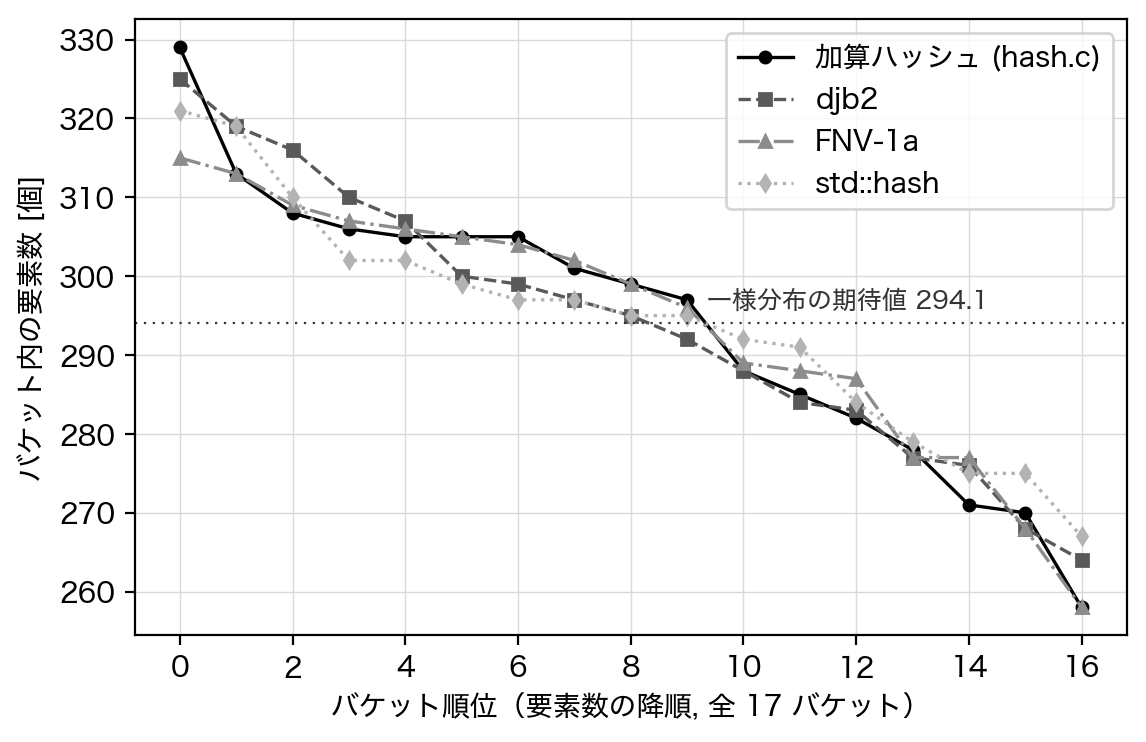
\includegraphics[width=0.8\linewidth]{../experiments/figures/collision_m17.png}
\caption{バケットごとの要素数分布（$m=17$，英単語 5000 語，要素数の降順）}
\label{fig:collision17}
\end{figure}

$m=17$ では 4 関数の差は小さい．いずれも $\chi^2$ 値は自由度 16 のカイ二乗分布の 5\% 点 26.3 を下回っており，統計的には一様分布と矛盾しない分布が得られている．なお {\tt std::hash} の具体的なアルゴリズムは処理系定義であり，本実験の {\tt stdhash} の数値は使用した処理系（Apple libc++）に固有である．すなわち，英単語のような自然なキー集合に対しては，$m$ が小さい間は加算ハッシュでも実用上十分な一様性をもつ．これは，単語の文字コード総和が数百から二千程度の広い範囲に分布し，それを小さな素数 17 で割った余りが十分に混ざるためと考えられる．

\subsubsection{表の大きさとハッシュ関数の相互作用}

ところが $m=1031$（素数）に拡大すると様相が一変する（図 \ref{fig:collision1031}，表 \ref{tab:collision1031}）．

\begin{table}[htbp]
\centering
\caption{ハッシュ関数ごとの衝突分布の要約（$m=1031$，$n=5000$）}
\label{tab:collision1031}
\begin{tabular}{lrrrr}
\hline
ハッシュ関数 & 空バケット数 & 最長チェイン & 分散 & $\chi^2$ 値 \\
\hline
加算ハッシュ & 57 & 20 & 14.54 & 3091.29 \\
djb2         & 7  & 13 & 4.67  & 991.76 \\
FNV-1a       & 6  & 12 & 4.78  & 1016.09 \\
{\tt std::hash} & 8 & 15 & 4.93 & 1048.26 \\
\hline
\end{tabular}
\end{table}

\begin{figure}[htbp]
\centering
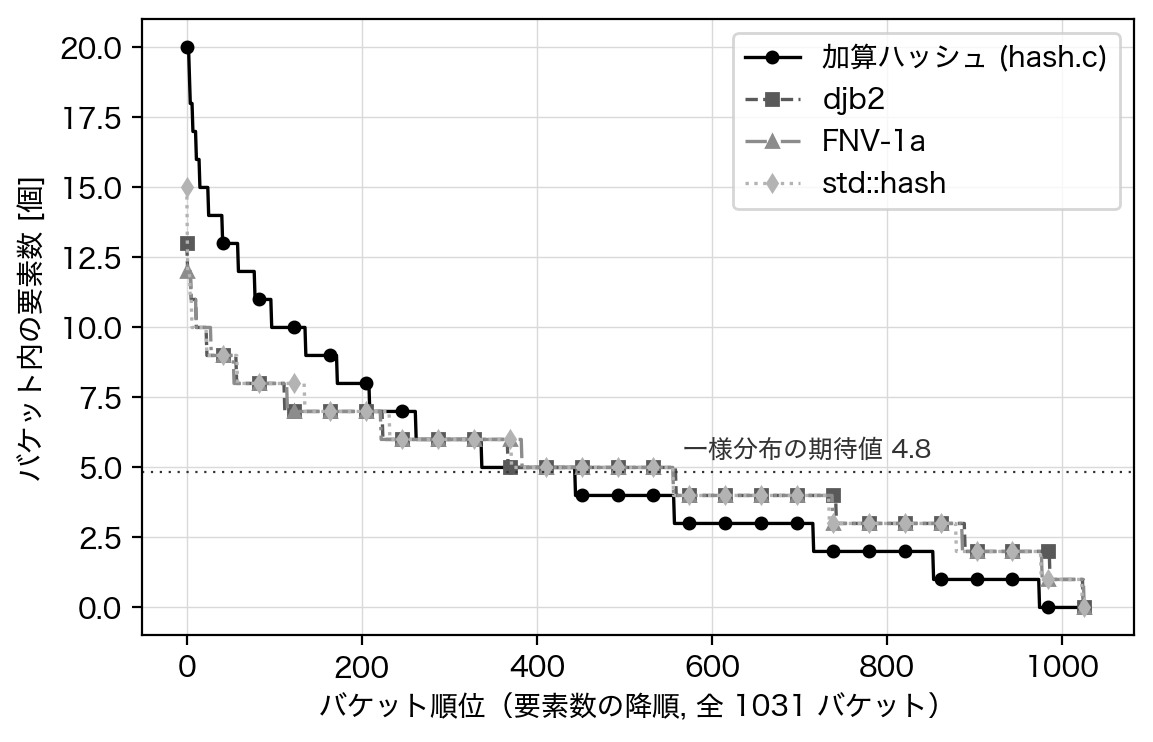
\includegraphics[width=0.8\linewidth]{../experiments/figures/collision_m1031.png}
\caption{バケットごとの要素数分布（$m=1031$，英単語 5000 語，要素数の降順）}
\label{fig:collision1031}
\end{figure}

自由度 1030 のカイ二乗分布の 5\% 点はおよそ 1106 であり，djb2・FNV-1a・{\tt std::hash} の $\chi^2$ 値（992〜1048）は一様分布と矛盾しないのに対し，加算ハッシュは 3091.29 と決定的に逸脱している．最長チェインも他の 1.5 倍以上，空バケットは 7 倍以上である．原因は，加算ハッシュの値域の狭さにある．英単語の文字コード総和は高々 2000 程度にしか達しないため，$m$ がこの値域と同程度以上になると，ハッシュ値が表の一部にしか届かず，剰余を取っても偏りが解消されない．すなわち加算ハッシュは「$m$ が小さいときに限り成立する」ハッシュ関数であり，表を大きくして性能を上げようとするとかえって偏りが顕在化する．この性質は，5.5 節で述べる動的リハッシュ（表の自動拡大）と致命的に相性が悪く，改良版でハッシュ関数の置き換えが必須であった理由である．

\subsubsection{表の大きさは素数でなければならないか}

2.2 節では「$m$ を素数にしておくと偏りの影響を受けにくい」と述べた．{\tt hash.c} の $m=17$ も {\tt std::unordered\_map} の実装も素数を用いる．この通説がハッシュ関数の品質とどう関係するかを確かめるため，同じ英単語 5000 語に対して，2 の冪とその近傍の素数の対（$m = 16/17$，$256/257$，$1024/1031$）で分布の統計量を比較した．結果を表 \ref{tab:tablesize} に示す．

\begin{table}[htbp]
\centering
\caption{バケット数 $m$（2 の冪と近傍の素数）による分布の比較（$n=5000$）}
\label{tab:tablesize}
\begin{tabular}{llrrrr}
\hline
ハッシュ関数 & $m$ & 空バケット数 & 最長チェイン & 分散 & $\chi^2$ 値 \\
\hline
加算ハッシュ & 16   & 0  & 353 & 284.62 & 14.57 \\
             & 17   & 0  & 329 & 311.16 & 17.99 \\
             & 256  & 0  & 32  & 20.44  & 267.87 \\
             & 257  & 0  & 33  & 20.84  & 275.28 \\
             & 1024 & 54 & 21  & 14.77  & 3097.79 \\
             & 1031 & 57 & 20  & 14.54  & 3091.29 \\
\hline
FNV-1a       & 16   & 0  & 339 & 244.00 & 12.49 \\
             & 17   & 0  & 315 & 253.75 & 14.67 \\
             & 256  & 0  & 31  & 19.89  & 260.70 \\
             & 257  & 0  & 31  & 17.91  & 236.63 \\
             & 1024 & 11 & 13  & 4.75   & 996.54 \\
             & 1031 & 6  & 12  & 4.78   & 1016.09 \\
\hline
\end{tabular}
\end{table}

この実験から 2 つの事実が読み取れる．第一に，加算ハッシュの破綻（$m=1024$ 以上での $\chi^2$ 値の急増）は $m$ が素数かどうかと無関係に起こる．$m=1024$ で 3097.79，素数の $m=1031$ でも 3091.29 であり，素数を選んでも救われない．5.2.2 節で述べたとおり破綻の原因はハッシュ値の値域の狭さであり，これは剰余の取り方では解消できないからである．第二に，FNV-1a は 2 の冪の $m$ でも近傍の素数と統計的に差のない一様性を示した（$m=1024$ で 996.54，$m=1031$ で 1016.09．自由度約 1000 のカイ二乗分布の 5\% 点は約 1100 であり，いずれも一様分布と矛盾しない）．

すなわち「$m$ は素数にせよ」という通説は，ハッシュ関数が弱い場合の防御策と理解するのが正確である．十分に撹拌するハッシュ関数を使うならば $m$ を 2 の冪に取ってよく，その場合，剰余演算 \% をビットマスク（論理積）に置き換えられるため，バケット番号の計算自体も高速化できる．実際，現代の高速ハッシュ表は除算を避ける工夫（2 の冪サイズや，乗算とシフトで剰余を代替する手法）を標準的に採用している \cite{munoz2022std}．ただし本実験のキーは英単語 1 種類のデータセットに限られるため，キーの構造によっては（例えば下位ビットに規則性をもつキー群では）2 の冪の $m$ が不利になり得ることには注意が必要である．

\subsubsection{アナグラム衝突}

加算ハッシュのもう 1 つの弱点は，文字の並び順を区別しないことである（2.2 節）．これを実験で確認した．表 \ref{tab:anagram} に，アナグラム関係にある 3 群のキーについて加算ハッシュと FNV-1a のバケット番号（$m=17$）を示す．

\begin{table}[htbp]
\centering
\caption{アナグラムキーに対するバケット番号の比較（$m=17$）}
\label{tab:anagram}
\begin{tabular}{lrr}
\hline
キー & 加算ハッシュ & FNV-1a \\
\hline
{\tt abc}    & 5 & 1 \\
{\tt acb}    & 5 & 1 \\
{\tt bac}    & 5 & 2 \\
{\tt bca}    & 5 & 1 \\
{\tt cab}    & 5 & 5 \\
{\tt cba}    & 5 & 4 \\
\hline
{\tt stop}   & 12 & 13 \\
{\tt tops}   & 12 & 7 \\
{\tt pots}   & 12 & 0 \\
{\tt spot}   & 12 & 3 \\
{\tt opts}   & 12 & 8 \\
{\tt post}   & 12 & 9 \\
\hline
{\tt listen} & 9 & 11 \\
{\tt silent} & 9 & 10 \\
{\tt enlist} & 9 & 5 \\
{\tt tinsel} & 9 & 12 \\
\hline
\end{tabular}
\end{table}

加算ハッシュでは 3 群とも全キーが同一バケットに集中し，最悪ケース（1 本のチェインへの集中）が容易に発生する．一方 FNV-1a は文字を読むたびに乗算で状態を撹拌するため並び順が結果に反映され，同じ 6 キーが 4〜6 個の異なるバケットに分散した．アナグラムは人工的な例に見えるが，「文字の構成が同じで並びだけ違うキー」は識別子やファイル名などで現実に生じ得る．さらに 5.7 節で述べるように，この性質は悪意ある入力に対する脆弱性に直結する．

\subsubsection{2020 年以降の知見との対応}

ハッシュ関数の品質評価は現在も活発な研究対象である．非暗号ハッシュ関数の標準的な品質検査系 SMHasher は雪崩性（入力 1 ビットの変化が出力の各ビットを確率 1/2 で反転させる性質）や分布の一様性を体系的に検査しており \cite{smhasher2024}，FNV-1a はこの検査で既知の弱点（雪崩性の不足など）が指摘される一方，簡潔さと十分な実用性能から今も広く使われている．より新しい wyhash 系の rapidhash（2024 年公開）は SMHasher 3 の全検査に合格した上で 64 バイト以下の短いキーに対して極めて高速であり \cite{rapidhash2024}，Rust 向けのベンチマーク比較でも短文字列キーに対する wyhash 系の優位が報告されている \cite{prodanov2023}．また 2024 年には CityHash64・MurmurHash2/3・wyhash などに対して，シードを知らなくても意図的に衝突を起こせる実用的な攻撃が公開されており \cite{orlp2024}，「速く一様である」ことと「敵対的入力に耐える」ことは別の要求であることが明確になっている．本課題の加算ハッシュは前者すら $m$ 依存でしか満たさない最も素朴な段階にあり，FNV-1a への置き換え（改良版）はこの発展系列の第一歩に位置づけられる．

\subsection{負荷率と探索性能について}

2.5 節の理論解析では，成功検索の平均比較回数は $1+\alpha/2$，不成功検索は $\alpha$ と見積もった（$\alpha$ は式 (\ref{eq:loadfactor}) の負荷率）．この理論値の妥当性を，$m=17$ 固定の表に英単語キーを $n=8$ 件から 1700 件（$\alpha = 0.47$ から 100）まで挿入して実測した．結果を図 \ref{fig:loadfactor} に示す．

\begin{figure}[htbp]
\centering
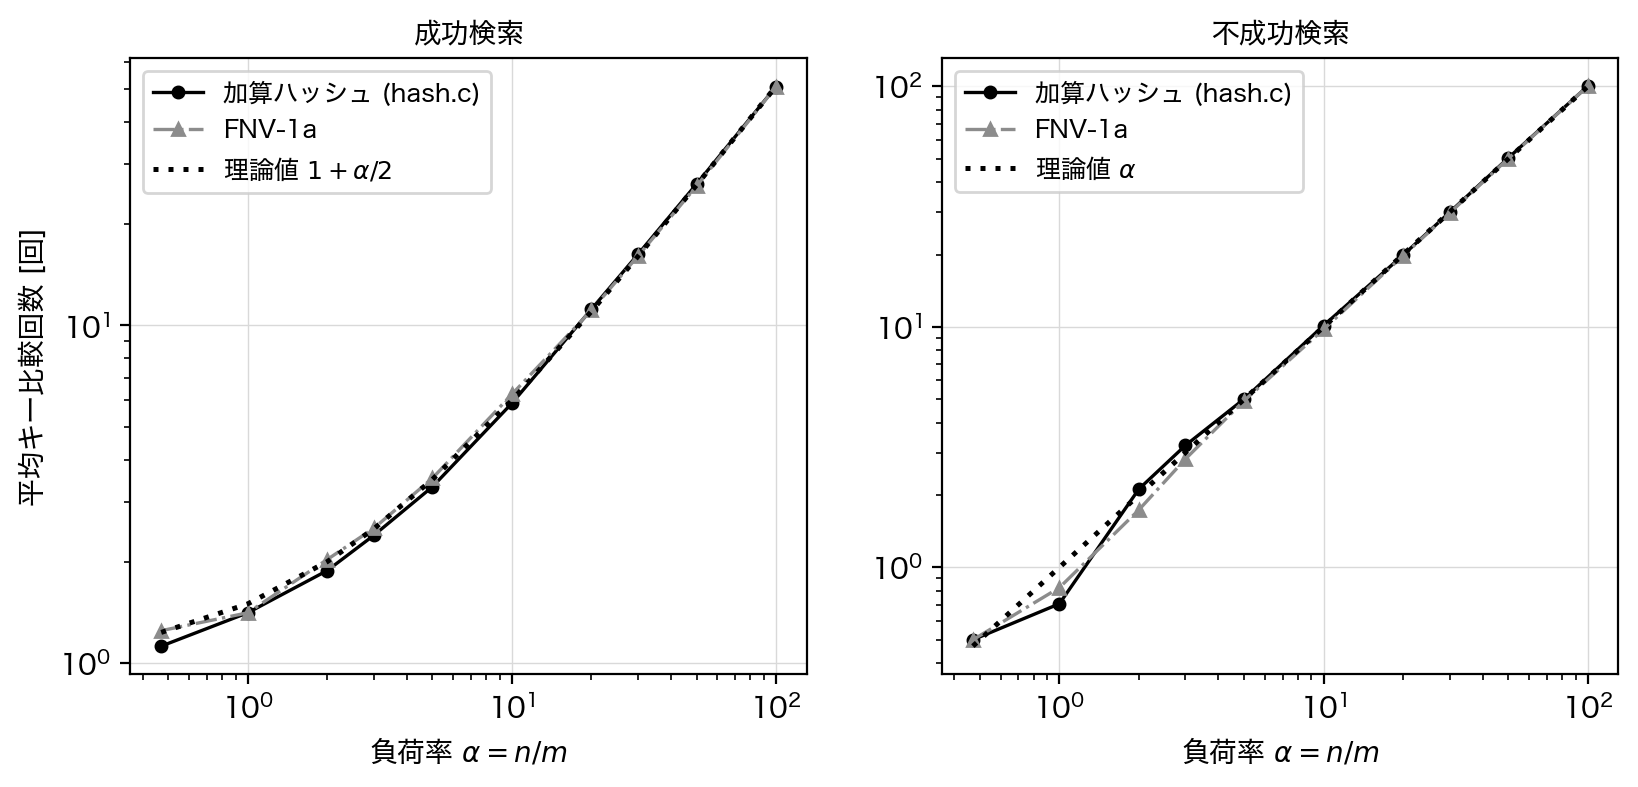
\includegraphics[width=\linewidth]{../experiments/figures/loadfactor.png}
\caption{負荷率 $\alpha$ と平均キー比較回数の関係（左: 成功検索，右: 不成功検索，両対数）}
\label{fig:loadfactor}
\end{figure}

実測値は理論値と極めてよく一致した．例えば加算ハッシュの成功検索は $\alpha=10$ で平均 5.88 回（理論値 6.0），$\alpha=100$ で 50.87 回（理論値 51.0）であり，誤差は 2\% 以内である．不成功検索も $\alpha=10$ で 10.13 回，$\alpha=100$ で 100.27 回と，理論値 $\alpha$ にほぼ重なる．FNV-1a でも同様であり（$\alpha=100$ で成功 50.83 回・不成功 100.30 回），$m=17$ においては両ハッシュ関数の差は誤差の範囲に収まる．これは 5.2.1 節で見たとおり $m=17$ では加算ハッシュも十分一様であることと整合する．

この結果は 2 つのことを意味する．第一に，単純一様ハッシュの仮定に基づく式 (\ref{eq:expected}) が，実在の英単語キーという「作為のない」入力に対して定量的に成立すること．第二に，バケット数固定のハッシュ表の探索コストは $\alpha$，すなわちデータ数に厳密に比例して劣化していくことである．$n=1700$（$\alpha=100$）の時点で成功検索に平均 51 回の文字列比較を要しており，これは連結リスト 1 本の線形探索（平均 850 回）よりは 17 倍速いものの，もはや「ほぼ一定時間」とは言えない．この観察が次節の実行時間測定と 5.5 節の動的リハッシュの動機となる．

\subsection{実行時間について}

\subsubsection{測定方法}

比較回数（前節）ではなく実時間を測るため，固定シードの擬似乱数で生成した 12 文字の英数字キー $N$ 個（$N = 10^3$ から $10^6$ まで対数等間隔の 7 点）を用い，(1) $N$ 件の挿入に要する合計時間，(2) 挿入済みキーからランダムに選んだ 10 万回の検索の 1 回あたり平均時間，を計測した．比較対象は，提出版と同構成の {\tt fixed17}（加算ハッシュ・$m=17$ 固定），改良版 {\tt improved}（FNV-1a・動的リハッシュ），標準ライブラリの {\tt std::unordered\_map}（チェイン法）および {\tt std::map}（平衡二分探索木）の 4 構造である．時刻取得には {\tt std::chrono::steady\_clock} を用い，各条件を 5 回繰り返した中央値を採用した（全測定値は付録 B.7）．なおこの検索時間の測定対象は成功検索のみであり，不成功検索の挙動は比較回数・プローブ数の実験（5.3 節および 5.5.5 節）で扱う．{\tt fixed17} は $N > 10^5$ では 1 回の検索に平均約 3000 回の文字列比較を要し測定が現実的でないため $N \le 10^5$ までとした．コンパイルは最適化オプション {\tt -O2} を付して行い，検索結果が最適化で除去されないよう検索の成功回数を集計・出力する構成とした．

結果を表 \ref{tab:timing} および図 \ref{fig:timing-insert}，図 \ref{fig:timing-lookup} に示す．

\begin{table}[htbp]
\centering
\caption{要素数 $N$ に対する挿入・検索時間（5 回の中央値）}
\label{tab:timing}
\begin{tabular}{lrrr}
\hline
データ構造 & $N$ & 挿入合計 [ms] & 検索平均 [ns] \\
\hline
{\tt fixed17}       & $10^3$ & 0.035    & 567.9 \\
                    & $10^4$ & 0.306    & 3440.7 \\
                    & $10^5$ & 3.487    & 374498.1 \\
{\tt improved}      & $10^3$ & 0.052    & 133.7 \\
                    & $10^4$ & 0.592    & 37.6 \\
                    & $10^5$ & 13.283   & 27.8 \\
                    & $10^6$ & 1496.228 & 952.6 \\
{\tt std::unordered\_map} & $10^3$ & 0.054 & 26.6 \\
                    & $10^4$ & 0.783    & 28.3 \\
                    & $10^5$ & 20.205   & 31.6 \\
                    & $10^6$ & 3584.558 & 1321.6 \\
{\tt std::map}      & $10^3$ & 0.155    & 331.6 \\
                    & $10^4$ & 3.825    & 240.6 \\
                    & $10^5$ & 95.797   & 872.1 \\
                    & $10^6$ & 6074.825 & 12907.7 \\
\hline
\end{tabular}
\end{table}

\begin{figure}[htbp]
\centering
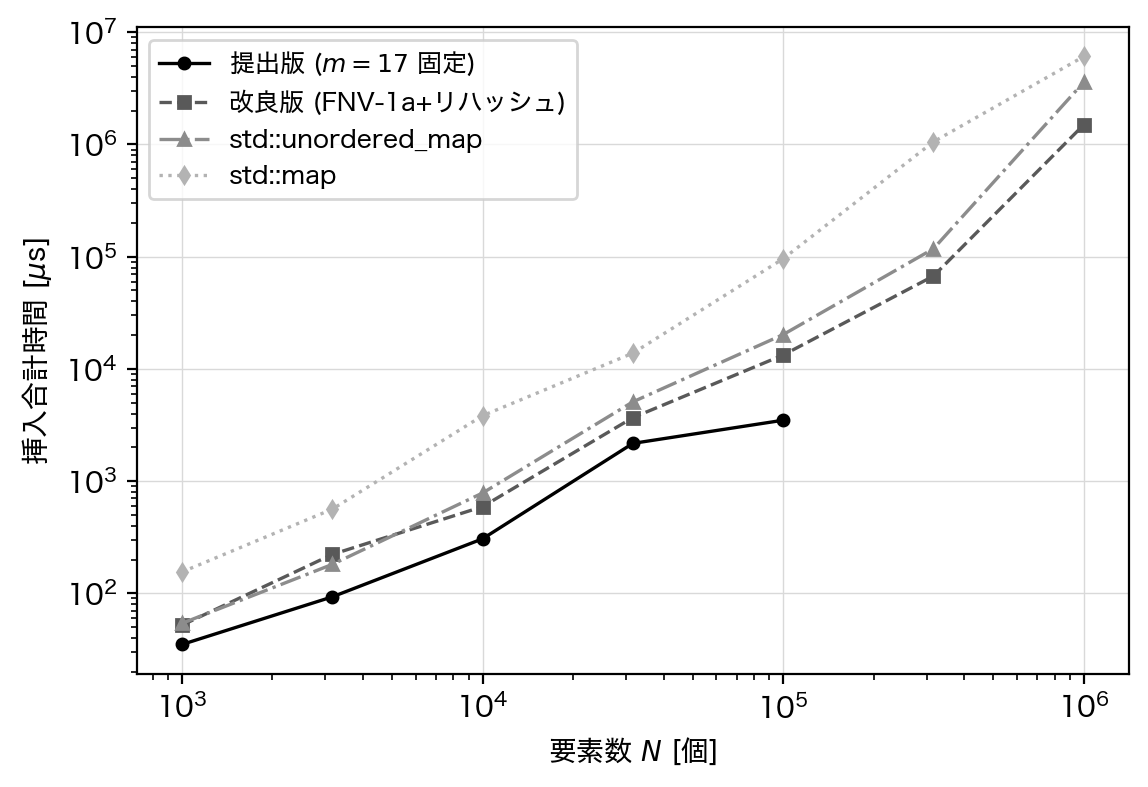
\includegraphics[width=0.8\linewidth]{../experiments/figures/timing_insert.png}
\caption{要素数 $N$ と挿入合計時間の関係（両対数，5 回の中央値）}
\label{fig:timing-insert}
\end{figure}

\begin{figure}[htbp]
\centering
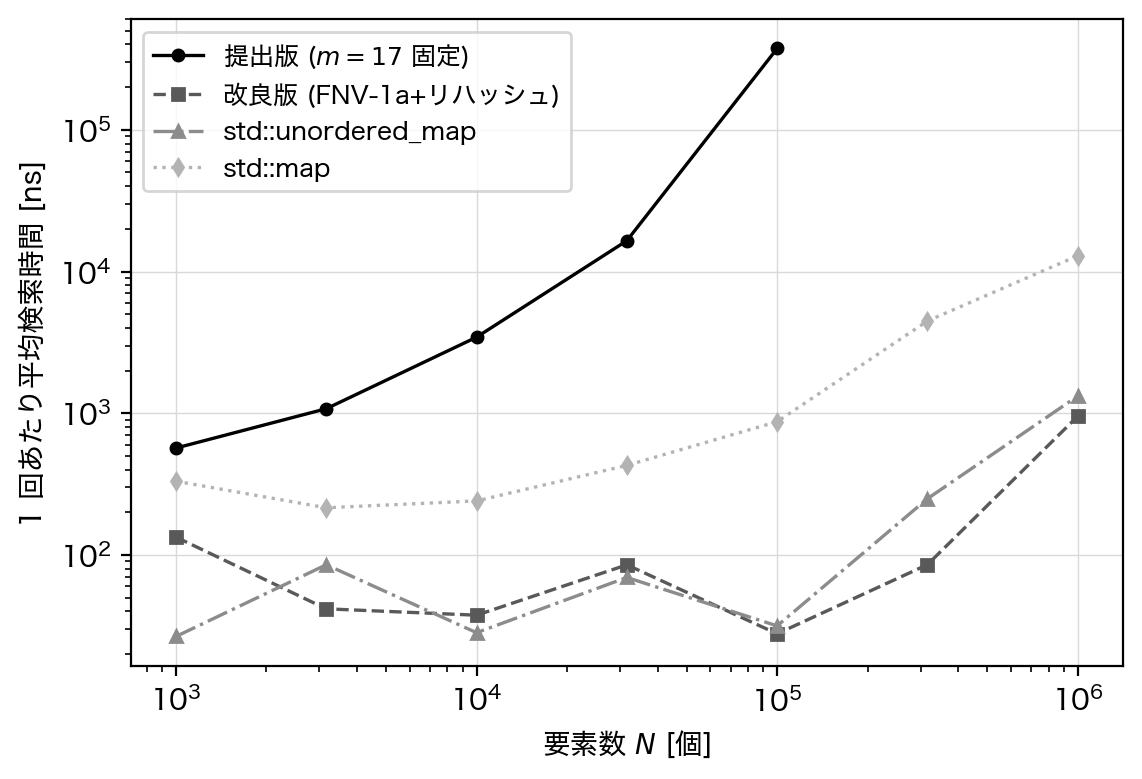
\includegraphics[width=0.8\linewidth]{../experiments/figures/timing_lookup.png}
\caption{要素数 $N$ と 1 回あたり平均検索時間の関係（両対数，5 回の中央値）}
\label{fig:timing-lookup}
\end{figure}

\subsubsection{提出版の性能特性}

{\tt fixed17} の検索時間は $N=10^3$ で 568 ns，$N=10^4$ で 3.44 $\mu$s，$N=10^5$ で 374 $\mu$s と，$N$ にほぼ比例して増加した．これは 5.3 節の比較回数の実験と整合し，バケット数固定のハッシュ表が漸近的には $O(N)$ の構造であることを実時間でも裏付けている．挿入は先頭挿入なので 1 件あたりほぼ一定（$N=10^5$ でも合計 3.5 ms）であり，「挿入は速いが検索が伸びる」という理論どおりの非対称性が観察された．

注目すべきは，検索時間の増加が比較回数の増加（$N$ に比例，100 倍）を上回る 659 倍に達している点である．1 ノードあたりの実時間に換算すると，$N=10^3$ では約 19 ns，$N=10^5$ では約 127 ns と 6 倍以上悪化している．チェインが長くなるとノード群がキャッシュに収まらなくなり，1 ノード辿るごとに主記憶アクセスが発生するためであり，5.5.2 節で述べる「比較回数の理論だけでは実時間を説明できない」というキャッシュ効率の問題を，本課題の規模でも定量的に観察できたことになる．

\subsubsection{改良版と標準ライブラリの比較}

{\tt improved} の検索時間は $N=10^4$〜$10^5$ で 30 ns 前後とほぼ一定であり，動的リハッシュによって負荷率が抑えられ，平均 $O(1)$ 検索が実時間でも成立している．$N=10^6$ で 953 ns へ増加するのは，表とノード群の総量が CPU キャッシュを超え，1 回の検索に伴うキャッシュミスが増えるためと考えられ，同じ増加傾向は {\tt std::unordered\_map}（31.6 ns $\rightarrow$ 1321.6 ns）にも現れている．

構造間の比較では，第一に，{\tt improved} は全域で {\tt std::unordered\_map} と同等以上の性能を示した．$N=10^6$ では挿入合計 1.50 s 対 3.58 s，検索平均 953 ns 対 1322 ns である．これは本実装が優れているというより，{\tt std::unordered\_map} が規格上の制約（要素のポインタ安定性等）を満たすための機構を抱えている\cite{munoz2022std}のに対し，本実装は機能を 3 操作に絞った単純な構造であることの帰結と解釈すべきである．第二に，{\tt std::map} は検索が $\log N$ に従って増加し（$N=10^6$ で 12.9 $\mu$s），$N=10^6$ における検索は {\tt improved} の約 13.5 倍遅い．キーの順序走査が不要で検索・挿入・削除だけが必要な用途では，ハッシュ表が平衡二分探索木より明確に有利であることが確認できた．

なお，個々の測定値には実行ごとに数倍程度のばらつきがあり（付録 B.7），これは測定を汎用 OS 上で行ったことによる他プロセスの影響が主因と考えられる．本考察では 5 回の中央値を用いることでこの影響を抑えた．また本測定では 4 構造を共通の仮想関数インタフェース越しに呼び出して条件を揃えているため，仮想関数呼び出しの固定費が全構造に一様に上乗せされている．この固定費は操作自体が軽い構造ほど相対的に大きく効くので，本実装と標準ライブラリの差は実際にはここで示した値よりわずかに開く方向にあると考えられる．

\subsubsection{キー長の影響}

ここまでの実験はキー長をほぼ一定（英単語または 12 文字）としてきたが，ハッシュ関数の計算量はキー長 $L$ に比例するため，長いキーでは様相が変わるはずである．キー長を 8 から 256 文字まで倍々に変えて，ハッシュ計算単体と成功検索の平均時間（15 回反復の最小値）を計測した．結果を図 \ref{fig:keylen} に示す．

\begin{figure}[htbp]
\centering
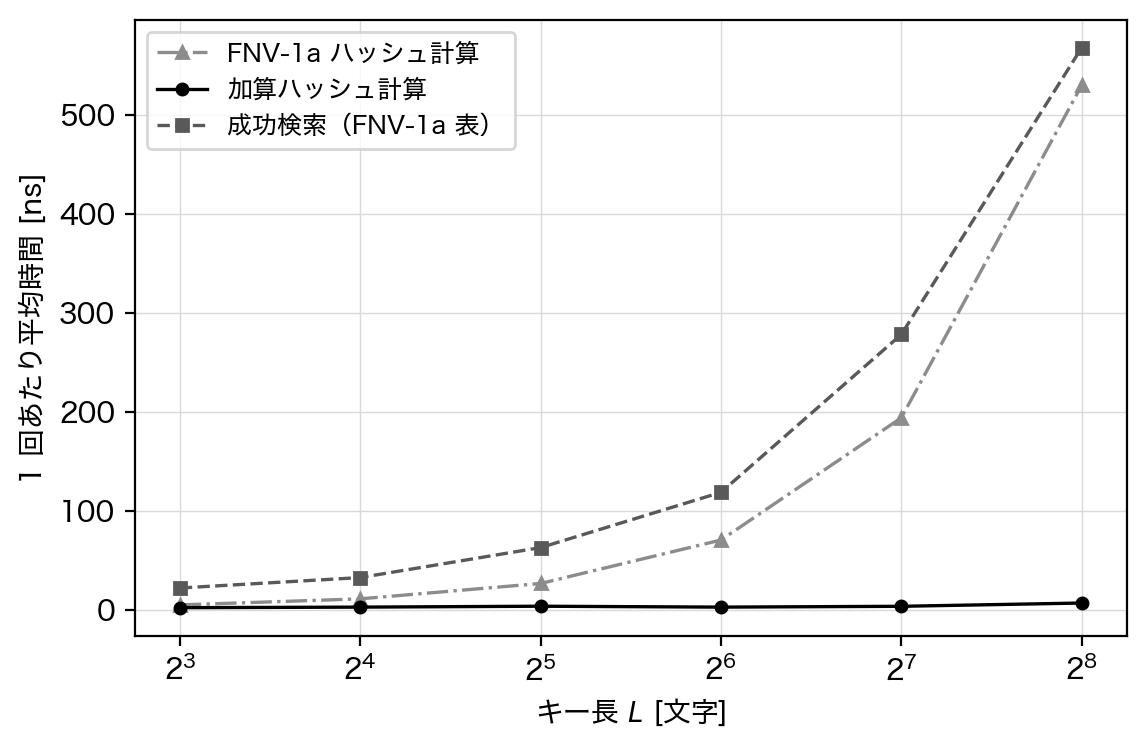
\includegraphics[width=0.8\linewidth]{../experiments/figures/keylen.png}
\caption{キー長 $L$ とハッシュ計算・検索時間の関係（$n=10000$，15 回反復の最小値）}
\label{fig:keylen}
\end{figure}

FNV-1a の計算時間は $L=8$ で 5.0 ns，$L=64$ で 70.6 ns，$L=256$ で 529.9 ns と，おおむね $L$ に比例して増加した．一方，加算ハッシュは $L=256$ でも 6.9 ns とほぼ一定のままである．この差は品質と速度のトレードオフの構造を示している．加算ハッシュの総和計算は繰返し間に依存関係がないためコンパイラが SIMD 命令で並列化できるのに対し，FNV-1a は「排他的論理和してから乗算」の結果が次の文字の計算に必要という逐次依存をもつため，1 文字ずつしか進められない．5.2 節で見た撹拌の良さは，まさにこの逐次的な混ぜ込みから来ているので，両者は表裏の関係にある．検索時間はキーが長くなるとハッシュ計算に支配され，$L=256$ では 567.9 ns 中の約 530 ns（9 割超）がハッシュ計算である．

この観察は，2020 年代のハッシュ関数が採る設計をよく説明する．wyhash 系の rapidhash などは，キーを 16〜48 バイト単位のブロックで読み，ブロック内は並列に処理できる乗算の構造を使うことで，逐次依存の連鎖を断ちつつ撹拌を保つ \cite{rapidhash2024,prodanov2023}．すなわち「品質は保ったまま並列性を回復する」ことが長いキーへの現代的な答えである．本実装の範囲でも，ノードにハッシュ値を保存しておきリハッシュ時の再計算を省く，比較の前にハッシュ値のタグで棄却する，といった「ハッシュ計算・比較の回数自体を減らす」改良が，長いキーに対して特に効果的になると考えられる．

\subsection{2020 年以降の知見に基づく改良について}

\subsubsection{改良版の設計}

以上の実験結果と近年の文献を踏まえ，2 点の改良を加えた {\tt hashtable\_improved.cpp} を作成した．
第一の改良はハッシュ関数の FNV-1a への置き換えである．5.2 節で示したとおり，加算ハッシュは表の拡大とともに偏りが顕在化するため，表の大きさによらず一様性を保つハッシュ関数が必要である．FNV-1a は 1 文字あたり排他的論理和 1 回と乗算 1 回という最小限の計算で実用的な一様性を達成し（表 \ref{tab:collision1031}），実装も 5 行程度と教育的な文脈でも見通しがよい．
第二の改良は動的リハッシュである．負荷率が 1.0 を超えた時点でバケット数を「現在の 2 倍以上で最小の素数」（$17 \rightarrow 37 \rightarrow 79 \rightarrow \cdots$）に拡張し全要素を再配置することで，$\alpha$ を常に一定以下に保ち，平均探索コストを式 (\ref{eq:expected}) の意味で $O(1)$ に維持する．拡張のたびに全要素の再配置（$O(n)$）が発生するが，表の大きさが等比数列的に成長するため，挿入 1 回あたりに均した償却コストは定数に収まる．これは 4.4 節で確認した拡張列と一致する．

この 2 つの改良が連動している点が本質的である．リハッシュだけを加算ハッシュのまま導入すると，$m$ が大きくなった時点で 5.2.2 節の偏りが現れ，負荷率を下げてもチェインが短くならないという形で破綻する．すなわち「よいハッシュ関数」は「表の成長」の前提条件である．リハッシュ処理の流れを図 \ref{fig:flow-rehash} に示す．

\begin{figure}[htbp]
\centering
\begin{tikzpicture}[node distance=8mm,
  startstop/.style={rectangle, rounded corners, draw, minimum width=30mm, minimum height=7mm},
  process/.style={rectangle, draw, minimum width=62mm, minimum height=7mm},
  decision/.style={diamond, aspect=2.4, draw, inner sep=1pt},
  arrow/.style={-{Stealth}}]
\node (start) [startstop] {挿入開始};
\node (d1) [decision, below=of start] {負荷率 $> 1.0$ か};
\node (p1) [process, below=of d1, yshift=-2mm] {$m' \leftarrow$ $2m$ 以上で最小の素数};
\node (p2) [process, below=of p1] {大きさ $m'$ の新バケット配列を確保};
\node (p3) [process, below=of p2] {全節を新しいハッシュ値の位置へ付け替え};
\node (p4) [process, below=of p3] {旧配列を解放し $m \leftarrow m'$};
\node (p5) [process, below=of p4] {通常の先頭挿入を実行};
\node (end) [startstop, below=of p5] {終了};
\draw [arrow] (start) -- (d1);
\draw [arrow] (d1) -- node[left] {はい} (p1);
\draw [arrow] (d1.east) -- node[above] {いいえ} +(24mm,0) |- (p5.east);
\draw [arrow] (p1) -- (p2);
\draw [arrow] (p2) -- (p3);
\draw [arrow] (p3) -- (p4);
\draw [arrow] (p4) -- (p5);
\draw [arrow] (p5) -- (end);
\end{tikzpicture}
\caption{改良版における動的リハッシュを含む挿入の流れ}
\label{fig:flow-rehash}
\end{figure}

\subsubsection{チェイン法の本質的限界とキャッシュ効率}

本課題のようなノードを {\tt new} で個別確保するチェイン法は，C++ 標準ライブラリの {\tt std::unordered\_map} と同系統の構造である．実は C++ 標準規格が要素へのポインタ安定性などを要求するため，{\tt std::unordered\_map} は事実上チェイン法での実装を強制されていることが知られている \cite{munoz2022std}．しかし 2020 年代の複数の大規模ベンチマークは，この方式が現代の計算機では不利であることを一致して報告している．Leitner-Ankerl による 29 実装の総合ベンチマーク（2022 年）では，{\tt std::unordered\_map} は検索・挿入・メモリ使用量のほぼ全項目で開放番地法系の実装に劣り \cite{ankerl2022bench}，Allan による 2024 年のベンチマークでも，表がキャッシュに収まらない規模ではチェインのノードを 1 つ辿るごとにキャッシュミスが 1 回発生することが劣位の主因と分析されている \cite{allan2024bench}．

この知見は本実装の性能特性の解釈に直結する．2.5 節の理論は「比較回数」を数えるが，現代の CPU では主記憶へのアクセス（キャッシュミス）1 回が数百命令分の時間に相当するため，同じ比較回数でもメモリ配置によって実時間は大きく変わる．チェイン法のノードはヒープ上に散在するため，チェインを辿る操作は本質的にキャッシュミスの連鎖である．比較回数の理論（図 \ref{fig:loadfactor}）が正確に成立してもなお，実時間では連続メモリ配置の構造に及ばないという二層構造を理解することが重要である．

\subsubsection{現代的ハッシュ表の設計動向}

チェイン法の限界に対する 2020 年代の主流の答えは，「要素を連続配列に直接格納し（開放番地法），ハッシュ値の一部をメタデータとして分離保存し，SIMD 命令で複数スロットを並列照合する」設計である．Boost 1.81（2022 年）で導入された {\tt boost::unordered\_flat\_map} は，15 スロットごとに 16 バイトのメタデータ語を持ち，縮約ハッシュ値を SSE2/Neon 命令で一括比較することで，1 回のメモリアクセスあたりの照合数を大幅に増やしている \cite{munoz2022flat}．同系統の設計は Google の Swiss Tables に始まり，Go 言語 1.24（2025 年）の組込み map にも採用された．Go の実装ではハッシュ値を上位 57 ビット（グループ選択用）と下位 7 ビット（メタデータ用）に分割し，8 スロット分の状態を 64 ビット制御語 1 つで並列照合することで，負荷率 7/8 まで性能劣化なく運用でき，マイクロベンチマークで最大 60\% の高速化を得たと報告されている \cite{gopratt2025}．Datadog はこの Go 1.24 の map への移行だけで単一サービスのヒープを約 500 MiB 削減したと報告しており \cite{datadog2025}，設計の違いが実運用のメモリ・速度に直接効くことがわかる．また Leitner-Ankerl の {\tt ankerl::unordered\_dense}（2022 年）は全要素を {\tt std::vector} に密に格納することで反復速度とメモリ効率を高めており \cite{unordereddense2022}，「ノードを個別確保しない」ことが共通の設計原理になっている．

本課題の実装をこの系譜に位置づけると，改良版（FNV-1a＋リハッシュ）は「ハッシュ関数の品質」と「負荷率の制御」までを解決した段階にあり，残る差分は「メモリ配置」である．さらなる改良としては，(1) ノードを可変長配列にまとめて確保しチェインを添字でつなぐ（キャッシュミス削減），(2) 各ノードにハッシュ値の下位バイトをタグとして保存し，文字列比較の前にタグ比較で棄却する（比較コスト削減，Swiss Tables の縮約ハッシュに相当），の 2 点が，クラスの外部仕様（{\tt ()}／{\tt insert}／{\tt -=}）を変えずに適用できる現実的な候補である．

\subsubsection{リハッシュの償却コストの実測}

動的リハッシュは「たまに全要素を再配置する」操作であるから，個々の挿入の所要時間は一様ではない．理論上は，表の大きさが等比数列的に成長する限り再配置の総仕事量は挿入数の定数倍に収まり，1 回あたりの償却コストは $O(1)$ となる．これを実測で確認するため，改良版と同じ構成の表に 20 万件のキーを挿入し，挿入 1 件ごとの所要時間を個別に記録した．結果を図 \ref{fig:rehash} に示す．

\begin{figure}[htbp]
\centering
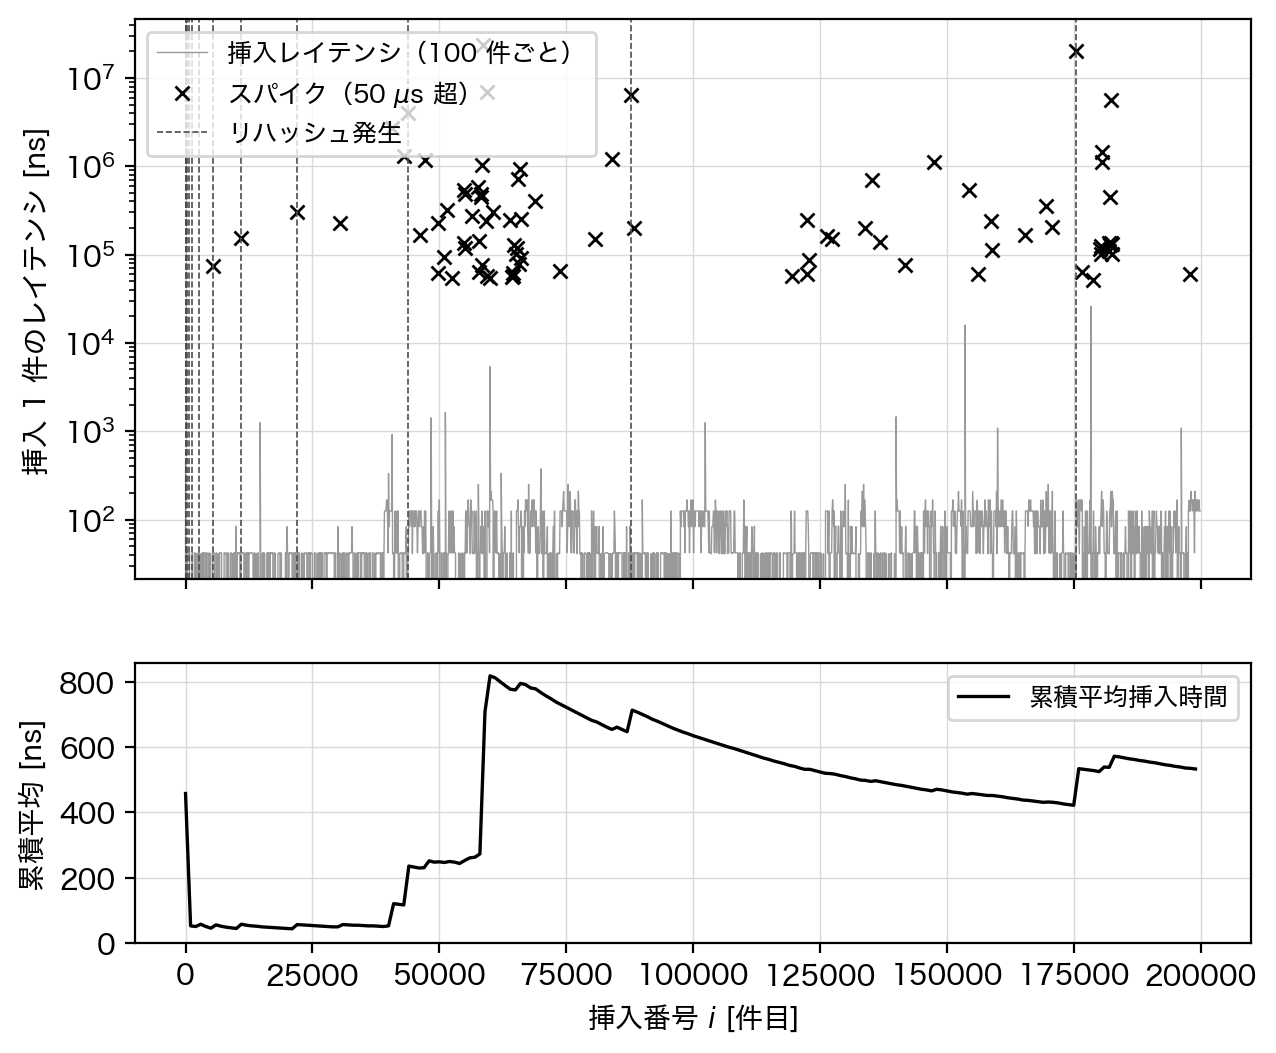
\includegraphics[width=0.95\linewidth]{../experiments/figures/rehash.png}
\caption{挿入レイテンシの時系列（上: 個別レイテンシと リハッシュ発生位置，対数軸）と累積平均挿入時間（下）（$N=200000$）}
\label{fig:rehash}
\end{figure}

20 万件の挿入中に発生したリハッシュの一覧を表 \ref{tab:rehashevents} に示す．リハッシュは 14 回発生し（バケット数は 17 から 350899 まで成長），挿入 1 件のレイテンシは最大 23.8 ms に達した．

\begin{table}[htbp]
\centering
\caption{20 万件挿入中に発生したリハッシュの一覧}
\label{tab:rehashevents}
\begin{tabular}{rr}
\hline
発生した挿入番号 & 新バケット数 \\
\hline
18     & 37 \\
38     & 79 \\
80     & 163 \\
164    & 331 \\
332    & 673 \\
674    & 1361 \\
1362   & 2729 \\
2730   & 5471 \\
5472   & 10949 \\
10950  & 21911 \\
21912  & 43853 \\
43854  & 87719 \\
87720  & 175447 \\
175448 & 350899 \\
\hline
\end{tabular}
\end{table}

このとき移動される節数はその時点の要素数（表 \ref{tab:rehashevents} の挿入番号にほぼ等しい）である．発生間隔とバケット数がともに等比数列的に増えている様子が読み取れる．これは通常の挿入（数十〜数百 ns）の数万倍である．それにもかかわらず全挿入の平均は 531 ns に収まった．図 \ref{fig:rehash} 下段の累積平均は，大きなスパイクの直後に段状に持ち上がるものの，その後に続く大量の高速な挿入によって押し下げられて収束していく．スパイク 1 回の仕事量（全要素の再配置）は表の成長とともに倍々に増えるが，発生間隔も倍々に開くため，平均への寄与が一定に抑えられるのである．これが償却 $O(1)$ の実体である．なお図中の 50 $\mu$s 超のスパイクにはリハッシュ発生位置（破線）と一致しないものも多数見られるが，これらは主にメモリ確保に伴う OS のページ割り当てなど測定環境側の要因と考えられ，リハッシュ由来の最大級のスパイク（ms 単位）とは規模が 1〜2 桁異なる．

この結果は同時に，動的リハッシュの限界も示している．平均は速くても，最悪の 1 回は 24 ms 止まるため，1 回ごとの応答時間に上限が要求される用途（対話処理や実時間制御）では，再配置を 1 度に行わず複数の操作に分割して漸進的に進める方式や，あらかじめ最終規模で表を確保しておく方式を検討する必要がある．償却計算量と最悪計算量の区別が実用上意味をもつことを示す好例といえる．

\subsubsection{開放番地法との比較実験}

2.3 節で述べたとおり，衝突処理にはチェイン法のほかに開放番地法があり，両方式の対比は近年の解説記事でも標準的な題材である \cite{zenn2023fika,qiita2025tachu}．5.5.3 節で見た現代的実装がすべて開放番地法系であることを踏まえ，両者の探索コストの性質の違いを自分の実装で確かめた．開放番地法として最も基本的な線形走査（衝突したら次のスロットを順に調べる方式，削除は墓標で表現）を FNV-1a と 2 の冪の容量で実装し，容量 131072 を固定して挿入数を変えることで負荷率 $\alpha$ を 0.25 から 0.95 まで制御し，成功・不成功検索の平均プローブ数（スロットまたはバケットの参照回数）を計測した．結果を図 \ref{fig:openaddr} に示す．図中の点線は理論値であり，チェイン法は成功 $1+\alpha/2$・不成功 $1+\alpha$，線形走査は成功 $\frac{1}{2}(1+\frac{1}{1-\alpha})$・不成功 $\frac{1}{2}(1+\frac{1}{(1-\alpha)^2})$ である（線形走査の式は Knuth による古典的解析として知られる）．

\begin{figure}[htbp]
\centering
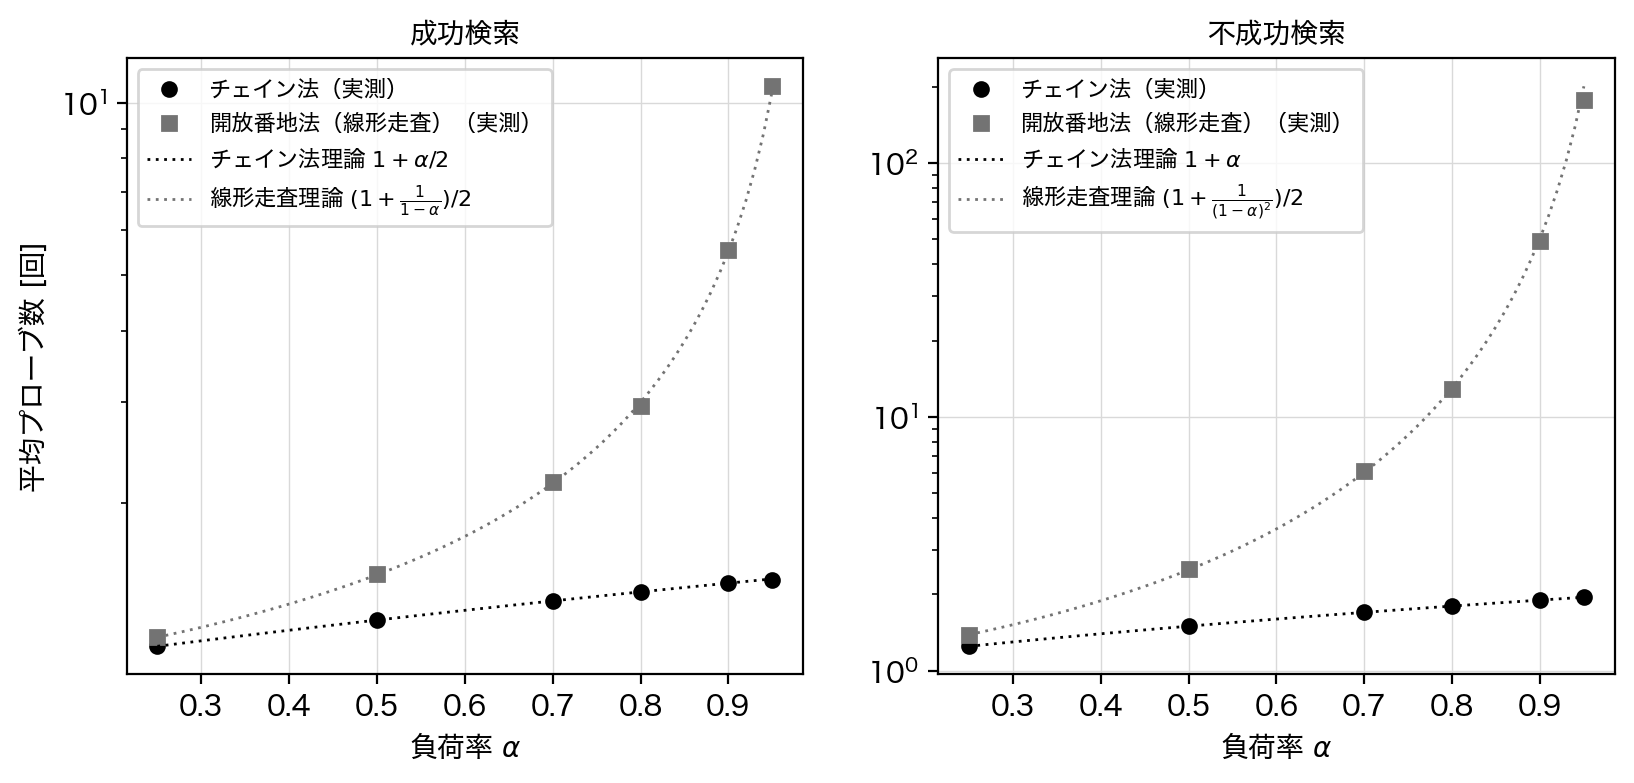
\includegraphics[width=\linewidth]{../experiments/figures/openaddr.png}
\caption{チェイン法と開放番地法（線形走査）の平均プローブ数の比較（左: 成功検索，右: 不成功検索，容量 131072）}
\label{fig:openaddr}
\end{figure}

実測は両方式とも理論値にほぼ完全に一致した．例えば $\alpha=0.9$ における線形走査の成功検索は実測 5.53 回（理論 5.50 回），不成功検索は実測 49.4 回（理論 50.5 回）である．プローブ数だけを見ると，チェイン法は $\alpha=0.95$ でも成功 1.47 回・不成功 1.95 回と穏やかに劣化するのに対し，線形走査は $\alpha \to 1$ で爆発的に悪化する（$\alpha=0.95$ で不成功 176.8 回）．衝突した要素が連続スロットを占有して塊（クラスタ）を作り，塊が大きいほどさらに衝突を吸い寄せるという正帰還が原因である．

この結果は一見，チェイン法の優位を示すように見える．それでも現代の高速実装が開放番地法を選ぶのは，プローブ 1 回あたりの実コストが桁違いに安いからである．線形走査のプローブは連続メモリ上の隣接スロットへの参照であり，多くはキャッシュに載っている．対してチェイン法のプローブはヒープ上に散在するノードへのポインタ追跡であり，1 回ごとにキャッシュミスを起こし得る（5.4.2 節で実測したとおり，チェインを 1 ノード辿る実時間は表の規模によって 19 ns から 127 ns まで変動した）．さらに実装側は負荷率に上限を課してプローブ数の爆発を防いでいる．{\tt boost::unordered\_flat\_map} は最大負荷率 0.875 \cite{munoz2022flat}，Go 1.24 の map は 7/8 \cite{gopratt2025} であり，図 \ref{fig:openaddr} の横軸でいえば爆発が始まる手前で必ずリハッシュする設計になっている．すなわち両方式の選択は「プローブ数で有利なチェイン法」対「プローブ単価で有利な開放番地法」のトレードオフであり，後者は負荷率制御という運用条件を追加することで成立している．

一方，本課題の仕様には削除 {\tt -=} が含まれるため，チェイン法の利点も明確である．チェイン法の削除はリストからの節の除去で完結するのに対し，開放番地法の削除は墓標（削除済み印）を残す必要があり，墓標が蓄積すると不成功検索がさらに劣化して定期的な作り直しが要る．3 操作が対等に要求される本課題の範囲では，チェイン法は実装の単純さと削除の素直さの点で妥当な選択であったと考えられる．

\subsubsection{タグ付き比較の実装と評価}

5.5.3 節で見た現代的設計のうち，チェイン法という枠組みを保ったまま適用できる要素として「縮約ハッシュの事前照合」がある．Swiss Tables 系の実装はハッシュ値の一部をメタデータとして保存し，本来のキー比較の前にこの短い値を照合して候補を絞り込む \cite{munoz2022flat,gopratt2025}．この着想をチェイン法に移植した発展版 {\tt hashtable\_tagged.cpp}（付録 A.14）を作成した．変更点は 3 つである．
第一に，節（{\tt Node}）に挿入時に計算した FNV-1a の 32 ビット値全体をタグとして保存する．
第二に，検索・削除のチェイン走査で，まず探索キーのハッシュ値と節のタグを整数比較し，一致したときに限り文字列比較を行う．
第三に，リハッシュ時には保存済みタグから新しいバケット番号を計算し，キー文字列の再ハッシュを行わない．
なお本実装の節は詰め物を含めて実質 48 バイト境界に丸められるため，タグ 4 バイトの追加は実メモリ消費を増やさない．

効果は，環境ノイズに左右されない決定的な指標として「検索 1 回あたりの文字列比較回数」で評価した（$N=200000$，$\alpha = 0.570$，10 万回検索）．結果を表 \ref{tab:tag} に示す．

\begin{table}[htbp]
\centering
\caption{タグ付き比較による文字列比較回数の削減（$N=200000$，$\alpha=0.570$，10 万回検索の平均）}
\label{tab:tag}
\begin{tabular}{llrr}
\hline
実装 & キー長 & 成功検索 [回/検索] & 不成功検索 [回/検索] \\
\hline
タグなし（改良版相当） & 12  & 1.28728 & 0.56954 \\
                       & 64  & 1.28554 & 0.56925 \\
                       & 256 & 1.28809 & 0.56863 \\
タグ付き               & 12  & 1.00000 & 0.00006 \\
                       & 64  & 1.00001 & 0.00007 \\
                       & 256 & 1.00002 & 0.00004 \\
\hline
\end{tabular}
\end{table}

タグなしの実測値は理論値（成功 $1+\alpha/2 = 1.285$，不成功 $\alpha = 0.570$）と一致する．タグ付きでは，成功検索の文字列比較が「一致する節の 1 回」だけに削減され，不成功検索ではほぼ完全にゼロ（10 万回あたり 4〜7 回）となった．残る数回は 32 ビットタグの偶然の一致であり，その確率はチェイン上の節 1 つあたり $2^{-32}$ 程度という見積もりと整合する．すなわち，不要な文字列比較という仕事そのものを原理的に消し去る改良であることが確認できた．また挿入（リハッシュ 14 回を含む）の合計時間は，キー再ハッシュの省略によりキー長 64 で 301 ms から 58 ms へと一貫して短縮された．一方，検索の実時間は本実験の規模では実行ごとのばらつき（OS のスケジューリングによる数倍の変動）に埋もれ，安定した差として観測できなかった．文字列比較 0.3 回分の削減は数 ns 規模であり，チェイン走査のキャッシュミス（数十〜百 ns）が支配的な本構造では，タグの真価はキー比較が高価な場合（長いキー，比較関数が重い型）や，メタデータを連続配置して SIMD で並列照合する段階（5.5.3 節）まで進んで初めて実時間に現れると考えられる．

\subsection{メモリ使用量について}

実行時間に加えて，メモリ使用量も構造選択の重要な判断軸である．12 文字のランダムキー $N$ 件の挿入前後でプロセスの最大常駐メモリ量（{\tt getrusage} の {\tt ru\_maxrss}）を測り，その増分を要素数で割った「1 要素あたりの増分メモリ」を比較した．結果を図 \ref{fig:memory} に示す．

\begin{figure}[htbp]
\centering
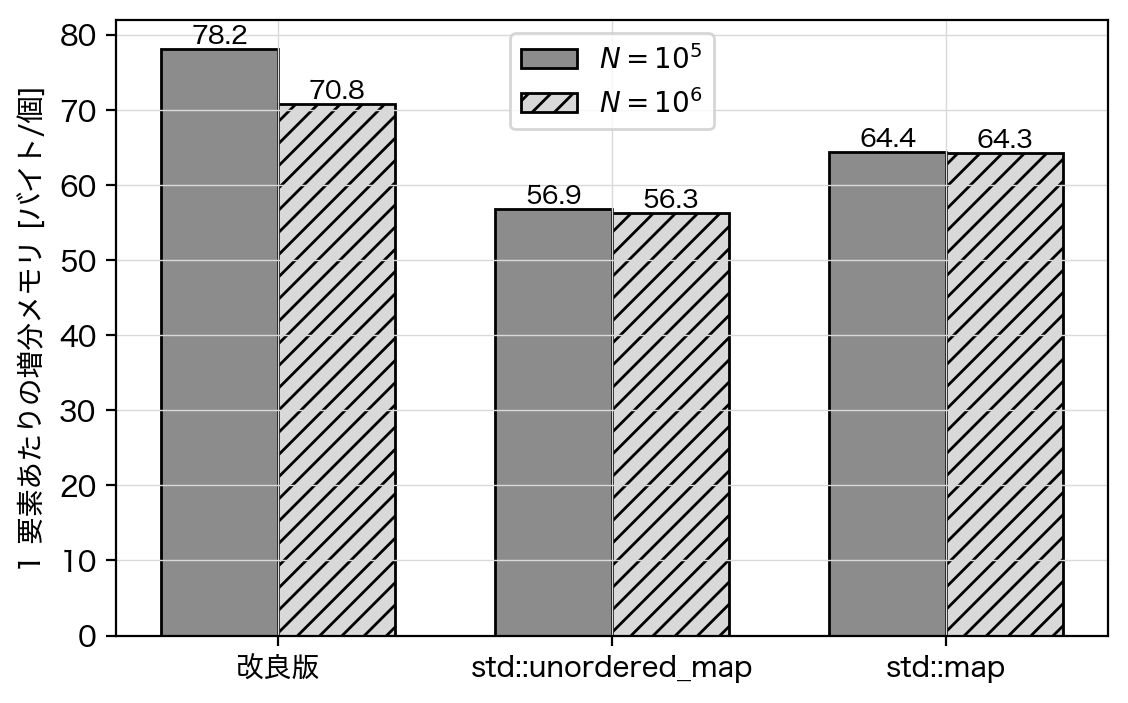
\includegraphics[width=0.75\linewidth]{../experiments/figures/memory.png}
\caption{1 要素あたりの増分メモリ使用量の比較（12 文字キー，値は {\tt int}）}
\label{fig:memory}
\end{figure}

$N=10^6$ における 1 要素あたりの増分は，改良版 70.8 バイト，{\tt std::unordered\_map} 56.3 バイト，{\tt std::map} 64.3 バイトであった．実行時間では優位だった改良版が，メモリでは最も多く消費している．この内訳は構造から説明できる．改良版のノードは {\tt std::string}（24 バイト）＋ {\tt int}（4 バイト＋詰め物 4 バイト）＋次ポインタ（8 バイト）の 40 バイトだが，メモリ確保器が 16 バイト境界に切り上げるため実質 48 バイトを占める．これにバケット配列（最終的に約 140 万バケット × 8 バイト $\approx$ 11 バイト/要素）が加わって約 59 バイト/要素となり，さらにリハッシュ中は新旧のバケット配列が一時的に共存して最大常駐量を押し上げる．残余は確保器の管理領域と考えられる．一方 {\tt std::map} の実測値 64.3 バイトは，キー・値対 32 バイト＋子ポインタ 2 本と親ポインタ・色情報 32 バイトという赤黒木ノードの理論値 64 バイトとほぼ一致する．

なお 12 文字のキーは {\tt std::string} の短文字列最適化（SSO）によりオブジェクト内に格納されるため，本測定にはキー本体のヒープ確保が含まれていない．キーが長い場合は全構造に同じだけの上乗せが生じる．ノードを個別確保するチェイン法がメモリ面でも不利になりやすいことは近年のベンチマークでも指摘されており \cite{allan2024bench}，全要素を連続領域に密に格納する設計 \cite{unordereddense2022} や，メタデータをビット単位に圧縮する設計 \cite{gopratt2025} がこの問題への現代的な回答である．実運用でもハッシュ表の内部設計の変更だけで数百 MiB 規模のメモリ削減が得られた事例が報告されている \cite{datadog2025}．

\subsection{ハッシュ表の安全性について}

5.2.4 節のアナグラム衝突は，性能問題であると同時に安全性の問題でもある．攻撃者が意図的に同一バケットへ衝突するキーを大量に送り込むと，ハッシュ表は 1 本の連結リストに退化し，操作あたり $O(n)$ の時間を消費させられる．これはハッシュ飽和攻撃（HashDoS）として知られ，Web サーバがリクエストパラメータをハッシュ表に格納する実装を狙った攻撃が現実に成立している \cite{sling2025}．加算ハッシュではアナグラムを列挙するだけで衝突キーを無限に生成できるため，本課題の提出版は敵対的環境では使用できない．

この攻撃が本課題の実装に対して実際に成立することを実験で確かめた．同一の文字マルチセット（{\tt a}〜{\tt d} 各 3 文字）の並べ替えからなる攻撃キー 2000 個と，通常のランダムキー 2000 個をそれぞれ挿入し，全キーの検索コストを計測した．結果を表 \ref{tab:hashdos} に示す．

\begin{table}[htbp]
\centering
\caption{ハッシュ飽和攻撃の実証（$n=2000$，検索 1 回あたりの平均）}
\label{tab:hashdos}
\begin{tabular}{llrrr}
\hline
実装 & キー群 & 最長チェイン & 平均比較回数 & 平均検索時間 [ns] \\
\hline
提出版（加算，$m=17$） & 攻撃キー     & 2000 & 1000.50 & 9656.94 \\
                       & ランダムキー & 144  & 59.89   & 250.43 \\
改良版（FNV-1a）       & 攻撃キー     & 5    & 1.36    & 31.26 \\
                       & ランダムキー & 5    & 1.38    & 30.75 \\
\hline
\end{tabular}
\end{table}

提出版では攻撃キー 2000 個の加算ハッシュ値がすべて一致してバケット 1 つに集中し（最長チェイン 2000），平均比較回数は 1000.50 回と，チェイン 1 本の線形探索の理論値 $(n+1)/2$ に正確に一致した．同じ要素数のランダムキー（59.89 回）と比べて約 17 倍，検索時間では約 39 倍の劣化である．攻撃者は要素数を増やすだけでこの劣化を際限なく深められる．一方，改良版では同じ攻撃キーが FNV-1a により 1416 バケットへ分散し（最長チェイン 5），比較回数はランダムキーと区別がつかない 1.36 回に留まった．すなわちアナグラム型の攻撃に対しては，ハッシュ関数の置き換えだけで防御が成立する．ただしこれは FNV-1a の衝突を作ることが加算ハッシュより難しいというだけであり，FNV-1a も鍵をもたない公開のアルゴリズムである以上，衝突キーを計算で列挙する攻撃は原理的に可能である．

現代の言語ランタイムはこの攻撃へのより根本的な対策として，鍵付きハッシュ関数 SipHash と実行ごとに変わる乱数シードを採用している．Rust の {\tt HashMap} は既定で SipHash-1-3 を用い \cite{sling2025}，Python の {\tt hash()} も文字列に対して起動ごとに異なるシードを混ぜるため，同じ文字列のハッシュ値が実行ごとに変わる \cite{chenna2023}．シードが秘密である限り攻撃者は衝突キーを事前計算できない．一方 2024 年の研究では，シードがあっても設計が弱いハッシュ関数（wyhash など）はシード非依存の衝突を構成できることが示されており \cite{orlp2024}，攻撃と防御の均衡は現在も動いている．理論面でも，攻撃下のハッシュ表の資源消費を保証付きで抑える手法が 2023 年に提案されるなど \cite{depthcharge2023}，ハッシュ表は完成した技術ではなく現役の研究対象である．本課題の文脈では，「ハッシュ関数は性能特性であると同時にセキュリティ境界である」という視点を，加算ハッシュという最も壊れやすい実例から学べたことが収穫である．

\subsection{C 版との設計比較}

最後に，出発点である {\tt hash.c} と本実装を設計の観点から比較する．

第一に資源管理である．{\tt hash.c} は {\tt malloc} で確保した節を一切解放せず，表の初期化も利用者が {\tt main} で明示的に行う．C++ 版はコンストラクタが初期化を，デストラクタが全節の解放を自動的に行うため，初期化忘れ・解放忘れが構文的に起こらない．これは C++ の RAII（資源確保は初期化時に）という設計原理の直接の恩恵である．

第二に安全性である．{\tt hash.c} の {\tt add} は {\tt strcpy(ptr->name, c)} で 16 バイト固定の配列にキーを複写するため，15 文字を超えるキーを渡すとバッファあふれ（未定義動作）が起こる．実際，本課題の実験で用いた英単語 5000 語には 16 文字以上の単語が含まれており，{\tt hash.c} をそのまま実験に流用することはできなかった．C++ 版はキーを {\tt std::string} で保持するため長さの制限自体が存在しない．C 言語でハッシュ表を実装する際の落とし穴と対策は近年の解説記事でも繰り返し指摘されており \cite{hoyt2021}，文字列の所有権管理は C 実装の主要な誤り源である．

第三に多重性と汎用性である．{\tt hash.c} の表はグローバル変数なのでプログラム中に 1 個しか存在できず，値の型も {\tt int} 固定である．C++ 版はオブジェクトなので必要なだけ生成でき，テンプレートにより任意の値型を収納できる（4.2 節で {\tt int}・{\tt double}・{\tt std::string} を確認）．

第四にインタフェースの表現力である．{\tt find(c)}・{\tt add(c, s)} という関数名ベースの C 版に対し，C++ 版は演算子多重定義により {\tt table("hoge")}・{\tt table -= "hoge"} という宣言的な記法を提供する．どちらが読みやすいかは文脈によるが，演算子という選択肢が言語機能として存在すること自体が，ライブラリの利用感を設計対象にできるという C++ の特徴である．

以上のとおり，同じアルゴリズム（チェイン法＋加算ハッシュ）であっても，実装言語の機構によって安全性・汎用性・保守性は大きく変わる．アルゴリズムの正しさ（2 節）とプログラムとしての堅牢さ（本節）は独立の関心事であり，後者において C++ の class は明確な利点を提供した．

\subsection{総括}

本課題で実装・評価した各版と標準ライブラリの特性を表 \ref{tab:summary} にまとめる．メモリの欄は 5.6 節の実測値（$N=10^6$，12 文字キー）である．

\begin{table}[htbp]
\centering
\caption{実装各版と標準ライブラリの特性のまとめ}
\label{tab:summary}
{\small
\begin{tabular}{llllll}
\hline
実装 & ハッシュ関数 & 表の成長 & 検索（平均） & メモリ & 主な限界 \\
     &              &          &              & [B/要素] & \\
\hline
提出版             & 加算       & なし（$m=17$） & $O(n/17)$ & --   & $n$ 増で線形劣化 \\
改良版             & FNV-1a     & 素数倍化      & $O(1)$    & 70.8 & 検索ごとのポインタ追跡 \\
発展版（タグ付き） & FNV-1a     & 素数倍化      & $O(1)$    & 70.8 & 同上（比較回数は削減） \\
{\tt std::unordered\_map} & 処理系定義 & 素数系列 & $O(1)$ & 56.3 & 規格制約による間接化 \\
{\tt std::map}     & --（比較木） & 平衡木        & $O(\log n)$ & 64.3 & キー比較が $\log n$ 回 \\
\hline
\end{tabular}
}
\end{table}

一連の実験を通じて得られた知見は次の 3 点に要約できる．
第一に，課題仕様の 3 操作（{\tt ()}・{\tt insert}・{\tt -=}）は，チェイン法により少ないコードで正しく実現でき，その正しさは理論（式 (\ref{eq:expected})）どおりの実測性能として定量的に裏付けられた．
第二に，素朴な実装と実用的な実装を分ける要素は，アルゴリズムの骨格ではなく「ハッシュ関数の品質」「負荷率の制御」「メモリ配置」という 3 つの工学的判断であり，それぞれの効果と限界を個別の実験（5.2 節，5.5.4 節，5.4.2 節）で切り分けて確認できた．
第三に，2020 年代の実装（Swiss Tables 系・{\tt boost::unordered\_flat\_map}・Go 1.24 の map）が到達している設計は，本課題の実装が抱える限界（ポインタ追跡・比較コスト・負荷率と性能の緊張関係）を段階的に解消してきた延長線上にあり，データ構造の教科書的な基礎と最先端の実装が地続きであることを実感できた．配列・リスト・木・ハッシュ表といった基本データ構造の得失を「何を解決し何を失うか」で整理する近年の視点 \cite{zenn2026tamai} に照らしても，本課題のハッシュ表は「検索の速さを得る代わりに順序とメモリ局所性を失う」構造として明確に位置づけられる．

今後の課題としては，(1) ノードの連続領域への配置によるキャッシュミス削減の実装と計測，(2) 上書き型 {\tt insert} への変更（5.1.4 節），(3) C++20 concepts によるテンプレート引数要求の明示（5.1.3 節），の 3 点が挙げられる．いずれも本レポートで確立した測定基盤（実験プログラム群と反復測定の手順）の上で定量評価が可能である．
